% ============================================================
%  Diagrama de Fluxo do Simulador de Máquinas Elétricas (EMS)
%
%  Uso em documento de duas colunas (IEEE / ABNT):
%
%  \begin{figure}
%    \centering
%    % ============================================================
%  Diagrama de Fluxo do Simulador de Máquinas Elétricas (EMS)
%
%  Uso em documento de duas colunas (IEEE / ABNT):
%
%  \begin{figure}
%    \centering
%    % ============================================================
%  Diagrama de Fluxo do Simulador de Máquinas Elétricas (EMS)
%
%  Uso em documento de duas colunas (IEEE / ABNT):
%
%  \begin{figure}
%    \centering
%    % ============================================================
%  Diagrama de Fluxo do Simulador de Máquinas Elétricas (EMS)
%
%  Uso em documento de duas colunas (IEEE / ABNT):
%
%  \begin{figure}
%    \centering
%    \input{diagrama_ems_fluxo.tex}
%    \caption{Fluxo de operação do Simulador de Máquinas
%             Elétricas (EMS).}
%    \label{fig:fluxo_ems}
%  \end{figure}
%
%  Árvore orientada de cima para baixo.
%  Sem sobreposição de caixas. Fundo branco.
%  Dimensionada para uma única coluna (~8.5 cm).
% ============================================================

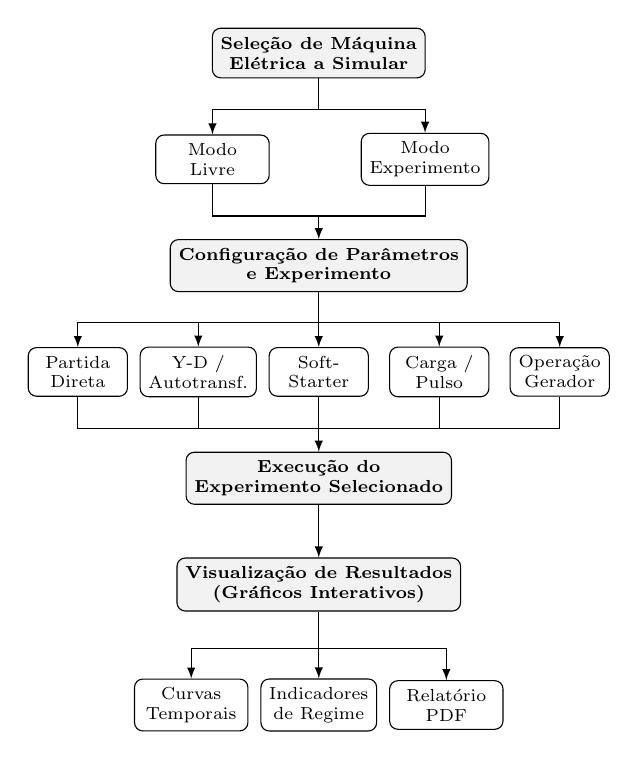
\begin{tikzpicture}[
    node distance=1.2cm and 0.4cm,
    scale=0.9, transform shape,
    % Nós comuns (folhas / intermediários)
    no/.style={
        draw,
        rounded corners=3pt,
        fill=white,
        font=\scriptsize,
        minimum width=1.6cm,
        minimum height=0.6cm,
        align=center
    },
    % Nós de destaque (marcos arquiteturais)
    nodest/.style={
        draw,
        rounded corners=3pt,
        fill=gray!10,
        font=\scriptsize\bfseries,
        minimum width=2.2cm,
        minimum height=0.7cm,
        align=center
    },
    linha/.style={draw, thin, -latex}
]

% ---- NÍVEL 0: RAIZ (CAPA DA APLICAÇÃO) ----
\node[nodest] (raiz) at (0, 0) {Seleção de Máquina\\Elétrica a Simular};

% ---- NÍVEL 1: MODOS DE OPERAÇÃO ----
\node[no] (m_livre) at (-1.5, -1.5) {Modo\\Livre};
\node[no] (m_exp)   at ( 1.5, -1.5) {Modo\\Experimento};

\coordinate (bif_modo) at (0, -0.8);
\draw[thin]  (raiz.south) -- (bif_modo);
\draw[linha] (bif_modo) -| (m_livre.north);
\draw[linha] (bif_modo) -| (m_exp.north);

% ---- NÍVEL 2: CONFIGURAÇÃO (CONVERGÊNCIA) ----
\node[nodest] (config) at (0, -3.0)
    {Configuração de Parâmetros\\e Experimento};

\coordinate (merge_modo) at (0, -2.3);
\draw[thin]  (m_livre.south) |- (merge_modo);
\draw[thin]  (m_exp.south)   |- (merge_modo);
\draw[linha] (merge_modo) -- (config.north);

% ---- NÍVEL 3: TIPOS DE EXPERIMENTO ----
\node[no, minimum width=1.4cm] (e1) at (-3.4, -4.5) {Partida\\Direta};
\node[no, minimum width=1.4cm] (e2) at (-1.7, -4.5) {Y-D /\\Autotransf.};
\node[no, minimum width=1.4cm] (e3) at ( 0.0, -4.5) {Soft-\\Starter};
\node[no, minimum width=1.4cm] (e4) at ( 1.7, -4.5) {Carga /\\Pulso};
\node[no, minimum width=1.4cm] (e5) at ( 3.4, -4.5) {Operação\\Gerador};

\coordinate (bif_e) at (0, -3.8);
\draw[thin]  (config.south) -- (bif_e);
\draw[linha] (bif_e) -| (e1.north);
\draw[linha] (bif_e) -| (e2.north);
\draw[linha] (bif_e) -- (e3.north);
\draw[linha] (bif_e) -| (e4.north);
\draw[linha] (bif_e) -| (e5.north);

% ---- NÍVEL 4: EXECUÇÃO (CONVERGÊNCIA) ----
\node[nodest] (sim) at (0, -6.0)
    {Execução do\\Experimento Selecionado};

\coordinate (merge_e) at (0, -5.3);
\draw[thin]  (e1.south) |- (merge_e);
\draw[thin]  (e2.south) |- (merge_e);
\draw[thin]  (e3.south) -- (merge_e);
\draw[thin]  (e4.south) |- (merge_e);
\draw[thin]  (e5.south) |- (merge_e);
\draw[linha] (merge_e) -- (sim.north);

% ---- NÍVEL 5: VISUALIZAÇÃO ----
\node[nodest] (vis) at (0, -7.5)
    {Visualização de Resultados\\(Gráficos Interativos)};

\draw[linha] (sim.south) -- (vis.north);

% ---- NÍVEL 6: ENTIDADES DOS RESULTADOS ----
\node[no, minimum width=1.6cm] (a1) at (-1.8, -9.2) {Curvas\\Temporais};
\node[no, minimum width=1.6cm] (a2) at ( 0.0, -9.2) {Indicadores\\de Regime};
\node[no, minimum width=1.6cm] (a3) at ( 1.8, -9.2) {Relatório\\PDF};

\coordinate (bif_a) at (0, -8.4);
\draw[thin]  (vis.south) -- (bif_a);
\draw[linha] (bif_a) -| (a1.north);
\draw[linha] (bif_a) -- (a2.north);
\draw[linha] (bif_a) -| (a3.north);

\end{tikzpicture}

%    \caption{Fluxo de operação do Simulador de Máquinas
%             Elétricas (EMS).}
%    \label{fig:fluxo_ems}
%  \end{figure}
%
%  Árvore orientada de cima para baixo.
%  Sem sobreposição de caixas. Fundo branco.
%  Dimensionada para uma única coluna (~8.5 cm).
% ============================================================

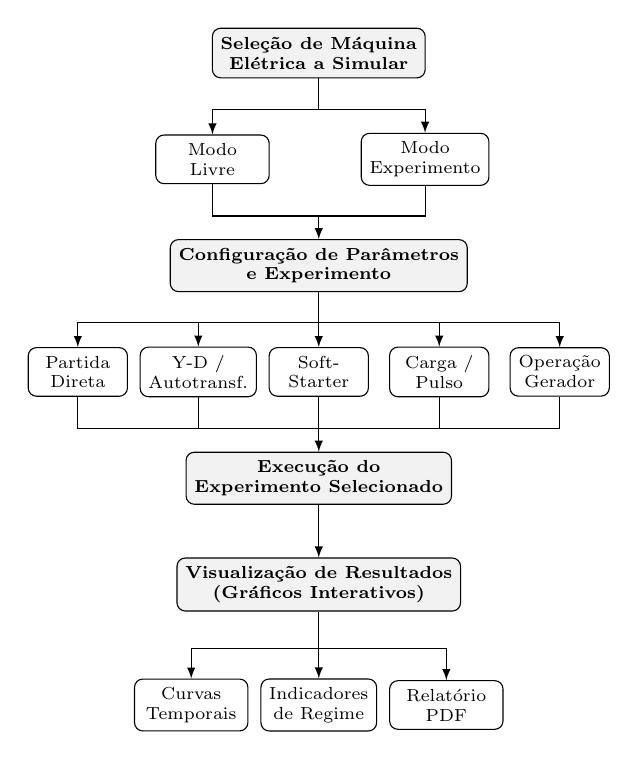
\begin{tikzpicture}[
    node distance=1.2cm and 0.4cm,
    scale=0.9, transform shape,
    % Nós comuns (folhas / intermediários)
    no/.style={
        draw,
        rounded corners=3pt,
        fill=white,
        font=\scriptsize,
        minimum width=1.6cm,
        minimum height=0.6cm,
        align=center
    },
    % Nós de destaque (marcos arquiteturais)
    nodest/.style={
        draw,
        rounded corners=3pt,
        fill=gray!10,
        font=\scriptsize\bfseries,
        minimum width=2.2cm,
        minimum height=0.7cm,
        align=center
    },
    linha/.style={draw, thin, -latex}
]

% ---- NÍVEL 0: RAIZ (CAPA DA APLICAÇÃO) ----
\node[nodest] (raiz) at (0, 0) {Seleção de Máquina\\Elétrica a Simular};

% ---- NÍVEL 1: MODOS DE OPERAÇÃO ----
\node[no] (m_livre) at (-1.5, -1.5) {Modo\\Livre};
\node[no] (m_exp)   at ( 1.5, -1.5) {Modo\\Experimento};

\coordinate (bif_modo) at (0, -0.8);
\draw[thin]  (raiz.south) -- (bif_modo);
\draw[linha] (bif_modo) -| (m_livre.north);
\draw[linha] (bif_modo) -| (m_exp.north);

% ---- NÍVEL 2: CONFIGURAÇÃO (CONVERGÊNCIA) ----
\node[nodest] (config) at (0, -3.0)
    {Configuração de Parâmetros\\e Experimento};

\coordinate (merge_modo) at (0, -2.3);
\draw[thin]  (m_livre.south) |- (merge_modo);
\draw[thin]  (m_exp.south)   |- (merge_modo);
\draw[linha] (merge_modo) -- (config.north);

% ---- NÍVEL 3: TIPOS DE EXPERIMENTO ----
\node[no, minimum width=1.4cm] (e1) at (-3.4, -4.5) {Partida\\Direta};
\node[no, minimum width=1.4cm] (e2) at (-1.7, -4.5) {Y-D /\\Autotransf.};
\node[no, minimum width=1.4cm] (e3) at ( 0.0, -4.5) {Soft-\\Starter};
\node[no, minimum width=1.4cm] (e4) at ( 1.7, -4.5) {Carga /\\Pulso};
\node[no, minimum width=1.4cm] (e5) at ( 3.4, -4.5) {Operação\\Gerador};

\coordinate (bif_e) at (0, -3.8);
\draw[thin]  (config.south) -- (bif_e);
\draw[linha] (bif_e) -| (e1.north);
\draw[linha] (bif_e) -| (e2.north);
\draw[linha] (bif_e) -- (e3.north);
\draw[linha] (bif_e) -| (e4.north);
\draw[linha] (bif_e) -| (e5.north);

% ---- NÍVEL 4: EXECUÇÃO (CONVERGÊNCIA) ----
\node[nodest] (sim) at (0, -6.0)
    {Execução do\\Experimento Selecionado};

\coordinate (merge_e) at (0, -5.3);
\draw[thin]  (e1.south) |- (merge_e);
\draw[thin]  (e2.south) |- (merge_e);
\draw[thin]  (e3.south) -- (merge_e);
\draw[thin]  (e4.south) |- (merge_e);
\draw[thin]  (e5.south) |- (merge_e);
\draw[linha] (merge_e) -- (sim.north);

% ---- NÍVEL 5: VISUALIZAÇÃO ----
\node[nodest] (vis) at (0, -7.5)
    {Visualização de Resultados\\(Gráficos Interativos)};

\draw[linha] (sim.south) -- (vis.north);

% ---- NÍVEL 6: ENTIDADES DOS RESULTADOS ----
\node[no, minimum width=1.6cm] (a1) at (-1.8, -9.2) {Curvas\\Temporais};
\node[no, minimum width=1.6cm] (a2) at ( 0.0, -9.2) {Indicadores\\de Regime};
\node[no, minimum width=1.6cm] (a3) at ( 1.8, -9.2) {Relatório\\PDF};

\coordinate (bif_a) at (0, -8.4);
\draw[thin]  (vis.south) -- (bif_a);
\draw[linha] (bif_a) -| (a1.north);
\draw[linha] (bif_a) -- (a2.north);
\draw[linha] (bif_a) -| (a3.north);

\end{tikzpicture}

%    \caption{Fluxo de operação do Simulador de Máquinas
%             Elétricas (EMS).}
%    \label{fig:fluxo_ems}
%  \end{figure}
%
%  Árvore orientada de cima para baixo.
%  Sem sobreposição de caixas. Fundo branco.
%  Dimensionada para uma única coluna (~8.5 cm).
% ============================================================

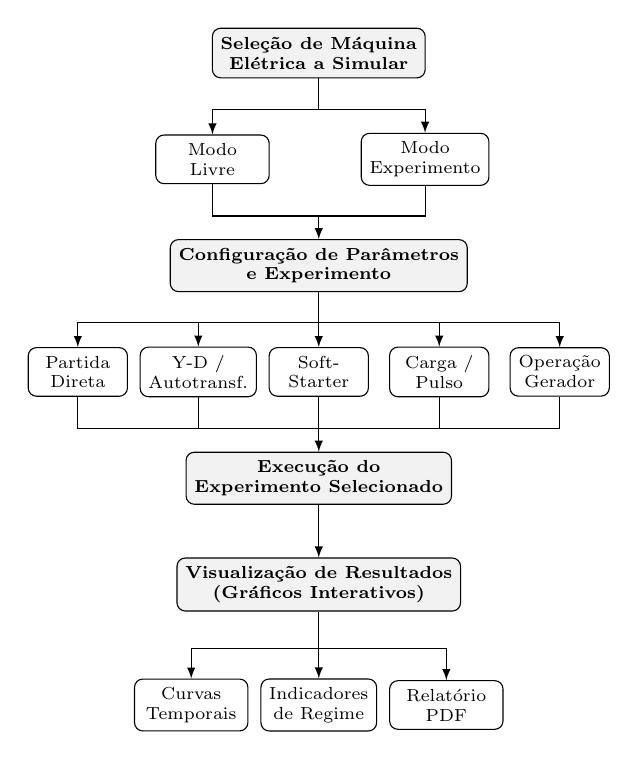
\begin{tikzpicture}[
    node distance=1.2cm and 0.4cm,
    scale=0.9, transform shape,
    % Nós comuns (folhas / intermediários)
    no/.style={
        draw,
        rounded corners=3pt,
        fill=white,
        font=\scriptsize,
        minimum width=1.6cm,
        minimum height=0.6cm,
        align=center
    },
    % Nós de destaque (marcos arquiteturais)
    nodest/.style={
        draw,
        rounded corners=3pt,
        fill=gray!10,
        font=\scriptsize\bfseries,
        minimum width=2.2cm,
        minimum height=0.7cm,
        align=center
    },
    linha/.style={draw, thin, -latex}
]

% ---- NÍVEL 0: RAIZ (CAPA DA APLICAÇÃO) ----
\node[nodest] (raiz) at (0, 0) {Seleção de Máquina\\Elétrica a Simular};

% ---- NÍVEL 1: MODOS DE OPERAÇÃO ----
\node[no] (m_livre) at (-1.5, -1.5) {Modo\\Livre};
\node[no] (m_exp)   at ( 1.5, -1.5) {Modo\\Experimento};

\coordinate (bif_modo) at (0, -0.8);
\draw[thin]  (raiz.south) -- (bif_modo);
\draw[linha] (bif_modo) -| (m_livre.north);
\draw[linha] (bif_modo) -| (m_exp.north);

% ---- NÍVEL 2: CONFIGURAÇÃO (CONVERGÊNCIA) ----
\node[nodest] (config) at (0, -3.0)
    {Configuração de Parâmetros\\e Experimento};

\coordinate (merge_modo) at (0, -2.3);
\draw[thin]  (m_livre.south) |- (merge_modo);
\draw[thin]  (m_exp.south)   |- (merge_modo);
\draw[linha] (merge_modo) -- (config.north);

% ---- NÍVEL 3: TIPOS DE EXPERIMENTO ----
\node[no, minimum width=1.4cm] (e1) at (-3.4, -4.5) {Partida\\Direta};
\node[no, minimum width=1.4cm] (e2) at (-1.7, -4.5) {Y-D /\\Autotransf.};
\node[no, minimum width=1.4cm] (e3) at ( 0.0, -4.5) {Soft-\\Starter};
\node[no, minimum width=1.4cm] (e4) at ( 1.7, -4.5) {Carga /\\Pulso};
\node[no, minimum width=1.4cm] (e5) at ( 3.4, -4.5) {Operação\\Gerador};

\coordinate (bif_e) at (0, -3.8);
\draw[thin]  (config.south) -- (bif_e);
\draw[linha] (bif_e) -| (e1.north);
\draw[linha] (bif_e) -| (e2.north);
\draw[linha] (bif_e) -- (e3.north);
\draw[linha] (bif_e) -| (e4.north);
\draw[linha] (bif_e) -| (e5.north);

% ---- NÍVEL 4: EXECUÇÃO (CONVERGÊNCIA) ----
\node[nodest] (sim) at (0, -6.0)
    {Execução do\\Experimento Selecionado};

\coordinate (merge_e) at (0, -5.3);
\draw[thin]  (e1.south) |- (merge_e);
\draw[thin]  (e2.south) |- (merge_e);
\draw[thin]  (e3.south) -- (merge_e);
\draw[thin]  (e4.south) |- (merge_e);
\draw[thin]  (e5.south) |- (merge_e);
\draw[linha] (merge_e) -- (sim.north);

% ---- NÍVEL 5: VISUALIZAÇÃO ----
\node[nodest] (vis) at (0, -7.5)
    {Visualização de Resultados\\(Gráficos Interativos)};

\draw[linha] (sim.south) -- (vis.north);

% ---- NÍVEL 6: ENTIDADES DOS RESULTADOS ----
\node[no, minimum width=1.6cm] (a1) at (-1.8, -9.2) {Curvas\\Temporais};
\node[no, minimum width=1.6cm] (a2) at ( 0.0, -9.2) {Indicadores\\de Regime};
\node[no, minimum width=1.6cm] (a3) at ( 1.8, -9.2) {Relatório\\PDF};

\coordinate (bif_a) at (0, -8.4);
\draw[thin]  (vis.south) -- (bif_a);
\draw[linha] (bif_a) -| (a1.north);
\draw[linha] (bif_a) -- (a2.north);
\draw[linha] (bif_a) -| (a3.north);

\end{tikzpicture}

%    \caption{Fluxo de operação do Simulador de Máquinas
%             Elétricas (EMS).}
%    \label{fig:fluxo_ems}
%  \end{figure}
%
%  Árvore orientada de cima para baixo.
%  Sem sobreposição de caixas. Fundo branco.
%  Dimensionada para uma única coluna (~8.5 cm).
% ============================================================

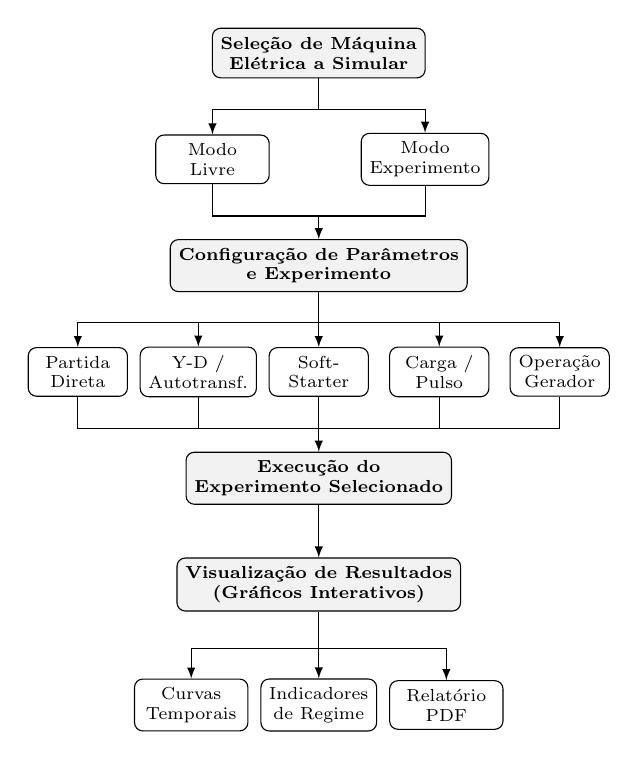
\begin{tikzpicture}[
    node distance=1.2cm and 0.4cm,
    scale=0.9, transform shape,
    % Nós comuns (folhas / intermediários)
    no/.style={
        draw,
        rounded corners=3pt,
        fill=white,
        font=\scriptsize,
        minimum width=1.6cm,
        minimum height=0.6cm,
        align=center
    },
    % Nós de destaque (marcos arquiteturais)
    nodest/.style={
        draw,
        rounded corners=3pt,
        fill=gray!10,
        font=\scriptsize\bfseries,
        minimum width=2.2cm,
        minimum height=0.7cm,
        align=center
    },
    linha/.style={draw, thin, -latex}
]

% ---- NÍVEL 0: RAIZ (CAPA DA APLICAÇÃO) ----
\node[nodest] (raiz) at (0, 0) {Seleção de Máquina\\Elétrica a Simular};

% ---- NÍVEL 1: MODOS DE OPERAÇÃO ----
\node[no] (m_livre) at (-1.5, -1.5) {Modo\\Livre};
\node[no] (m_exp)   at ( 1.5, -1.5) {Modo\\Experimento};

\coordinate (bif_modo) at (0, -0.8);
\draw[thin]  (raiz.south) -- (bif_modo);
\draw[linha] (bif_modo) -| (m_livre.north);
\draw[linha] (bif_modo) -| (m_exp.north);

% ---- NÍVEL 2: CONFIGURAÇÃO (CONVERGÊNCIA) ----
\node[nodest] (config) at (0, -3.0)
    {Configuração de Parâmetros\\e Experimento};

\coordinate (merge_modo) at (0, -2.3);
\draw[thin]  (m_livre.south) |- (merge_modo);
\draw[thin]  (m_exp.south)   |- (merge_modo);
\draw[linha] (merge_modo) -- (config.north);

% ---- NÍVEL 3: TIPOS DE EXPERIMENTO ----
\node[no, minimum width=1.4cm] (e1) at (-3.4, -4.5) {Partida\\Direta};
\node[no, minimum width=1.4cm] (e2) at (-1.7, -4.5) {Y-D /\\Autotransf.};
\node[no, minimum width=1.4cm] (e3) at ( 0.0, -4.5) {Soft-\\Starter};
\node[no, minimum width=1.4cm] (e4) at ( 1.7, -4.5) {Carga /\\Pulso};
\node[no, minimum width=1.4cm] (e5) at ( 3.4, -4.5) {Operação\\Gerador};

\coordinate (bif_e) at (0, -3.8);
\draw[thin]  (config.south) -- (bif_e);
\draw[linha] (bif_e) -| (e1.north);
\draw[linha] (bif_e) -| (e2.north);
\draw[linha] (bif_e) -- (e3.north);
\draw[linha] (bif_e) -| (e4.north);
\draw[linha] (bif_e) -| (e5.north);

% ---- NÍVEL 4: EXECUÇÃO (CONVERGÊNCIA) ----
\node[nodest] (sim) at (0, -6.0)
    {Execução do\\Experimento Selecionado};

\coordinate (merge_e) at (0, -5.3);
\draw[thin]  (e1.south) |- (merge_e);
\draw[thin]  (e2.south) |- (merge_e);
\draw[thin]  (e3.south) -- (merge_e);
\draw[thin]  (e4.south) |- (merge_e);
\draw[thin]  (e5.south) |- (merge_e);
\draw[linha] (merge_e) -- (sim.north);

% ---- NÍVEL 5: VISUALIZAÇÃO ----
\node[nodest] (vis) at (0, -7.5)
    {Visualização de Resultados\\(Gráficos Interativos)};

\draw[linha] (sim.south) -- (vis.north);

% ---- NÍVEL 6: ENTIDADES DOS RESULTADOS ----
\node[no, minimum width=1.6cm] (a1) at (-1.8, -9.2) {Curvas\\Temporais};
\node[no, minimum width=1.6cm] (a2) at ( 0.0, -9.2) {Indicadores\\de Regime};
\node[no, minimum width=1.6cm] (a3) at ( 1.8, -9.2) {Relatório\\PDF};

\coordinate (bif_a) at (0, -8.4);
\draw[thin]  (vis.south) -- (bif_a);
\draw[linha] (bif_a) -| (a1.north);
\draw[linha] (bif_a) -- (a2.north);
\draw[linha] (bif_a) -| (a3.north);

\end{tikzpicture}
